% !TeX spellcheck = it_IT
\newpage
\section{DBMS}
Un DBMS è un sistema software che gestisce grandi quantità di dati \textbf{persistenti} e \textbf{condivisi}. Questo implica che deve essere \textbf{efficiente} e garantire \textbf{affidabilità} (fault tolerance).
\begin{center}
	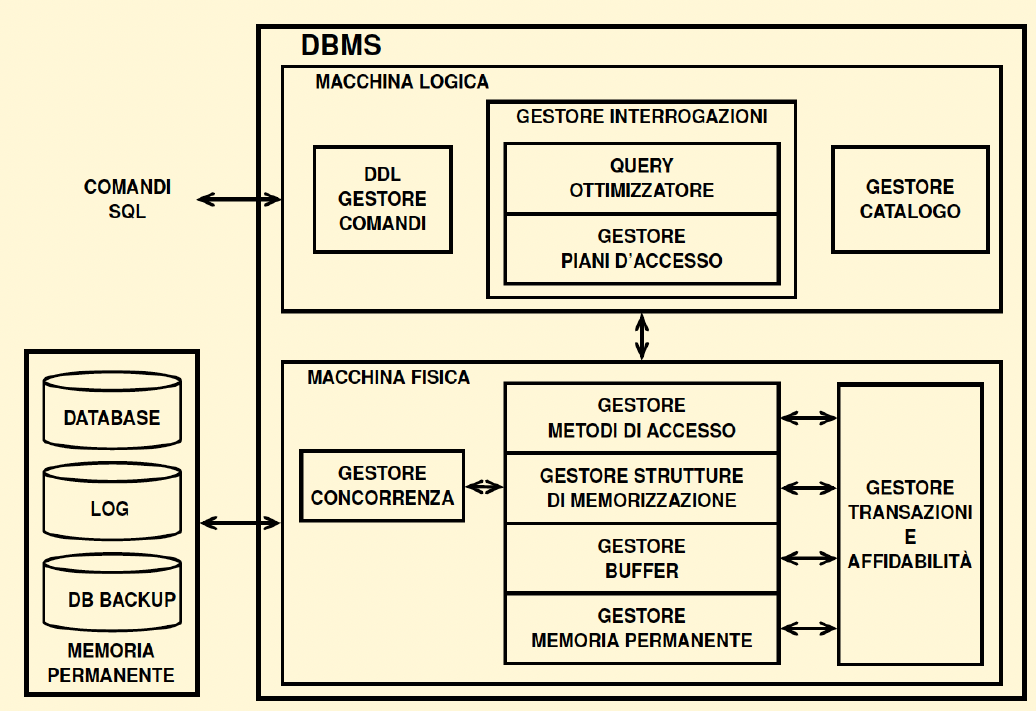
\includegraphics[scale=0.4]{dbms.png}
\end{center}

\subsection{Memorie}
La memoria di un sistema di calcolo organizzato è divisa in livelli: da quelle più piccole, costose e veloci a quelle grandi, economiche e lente.\\
Le prestazioni si misurano in \textbf{tempo di accesso}, che è determinato da \textbf{latenza} (tempo di accesso al primo byte) e \textbf{tempo di trasferimento} dei dati:
\begin{equation}
	T_{\text{accesso}} = \text{latenza} + \frac{\text{dimDati}}{\text{velTransfer}}
\end{equation}

\begin{center}
	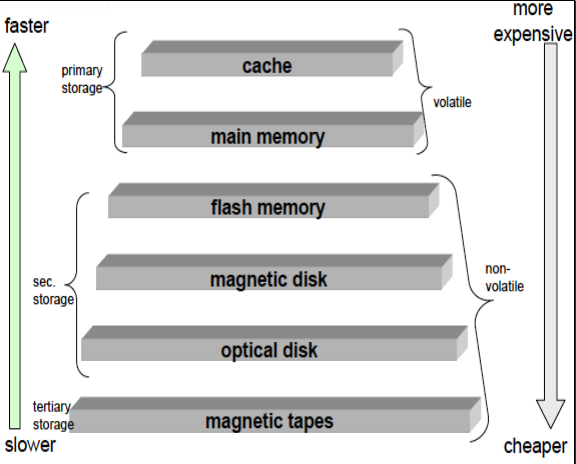
\includegraphics[scale=0.3]{memorie.png}
\end{center}
In una BD, considerate le dimensioni, risiede di solito su \textbf{dischi} e i dati vengono poi trasferiti a \textbf{blocchi} (o pagine) nella memoria centrale per essere elaborati.
\subsubsection{Hard disk}
Un hard disk (HD) è un dispositivo elettro-meccanico per la conservazione di informazioni sotto forma magnetica, su supporto rotante a forma di piatto su cui agiscono delle testine di lettura e scrittura.\\
Un’unità a dischi contiene una pila di dischi metallici che ruota a velocità costante ed alcune testine di lettura che si muovono radialmente al disco.
\begin{center}
	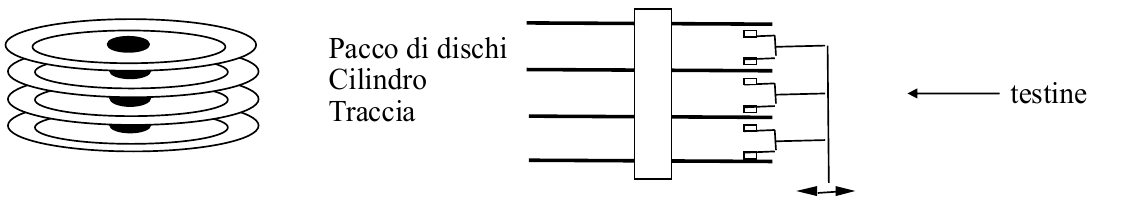
\includegraphics[scale=0.3]{hdd.png}
\end{center}
Una \textbf{traccia} è organizzata in \textbf{settori} di dimensione fissa. Questi sono a loro volta raggruppati logicamente in \textbf{blocchi}, che sono l'unità di trasferimento.

\begin{note}
	Negli hard disk è fondamentale la \textbf{località}: se i settori sono vicini si impiega molto meno tempo.
\end{note}

\subsubsection{Pagina}
Un blocco o pagina è una sequenza contigua di settori su una traccia e costituisce l'unità per il trasferimento dei dati. Tipicamente è grande da $4$KB a $64$KB. Più sono piccole e più operazioni servono ma più grandi sono è più serve tempo per caricarle e si rischia frammentazione.\\
Il \textbf{tempo di trasferimento} $T_t$ di una pagina dipende dalla dimensione della pagina $P$ e dal transfer rate $T_r$.\\
La struttura di una pagina si divide in:
\begin{itemize}
	\item \textbf{Fisica}: un insieme di dimensione fissa di caratteri
	\item \textbf{Logica}: contiene informazioni di servizio e le stringhe che rappresentano i record
\end{itemize}
In un DBMS la struttura tipica di una pagina è la seguente
\begin{center}
	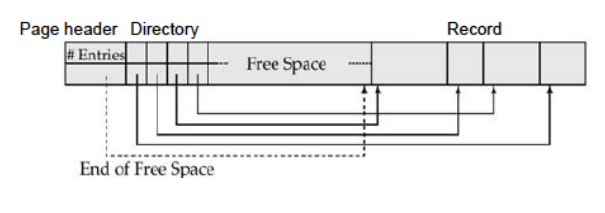
\includegraphics[scale=0.5]{pagina1.png}
\end{center}
La \textbf{directory} contiene un puntatore per ogni record nella pagina. In questo modo l'\textbf{identificatore di un record} (RID) nel DB è formato da:
\begin{itemize}
	\item \textbf{PID}: identificatore della pagina
	\item \textbf{Slot}: posizione all'interno della pagina
\end{itemize}
Garantendo così un'individuazione veloce e la riallocazione senza modifica del RID.
\begin{center}
	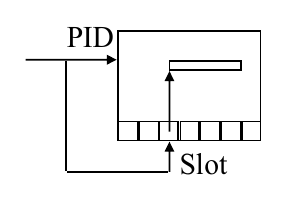
\includegraphics[scale=0.5]{pagina2.png}
\end{center}

\subsubsection{Gestore memoria permanente}
Fornisce un’\textbf{astrazione} della memoria permanente in termini di insiemi di file logici di pagine fisiche di registrazioni (blocchi), nascondendo le caratteristiche dei dischi e del sistema operativo.

\subsubsection{Gestore del buffer}
Il gestore del buffer si preoccupa del trasferimento delle pagine tra la memoria temporanea e la memoria permanente, offrendo una visione della memoria permanente come un insieme di pagine utilizzabili in memoria temporanea, astraendo da quando esse vengano trasferite dalla memoria permanente al buffer e viceversa.

\begin{center}
	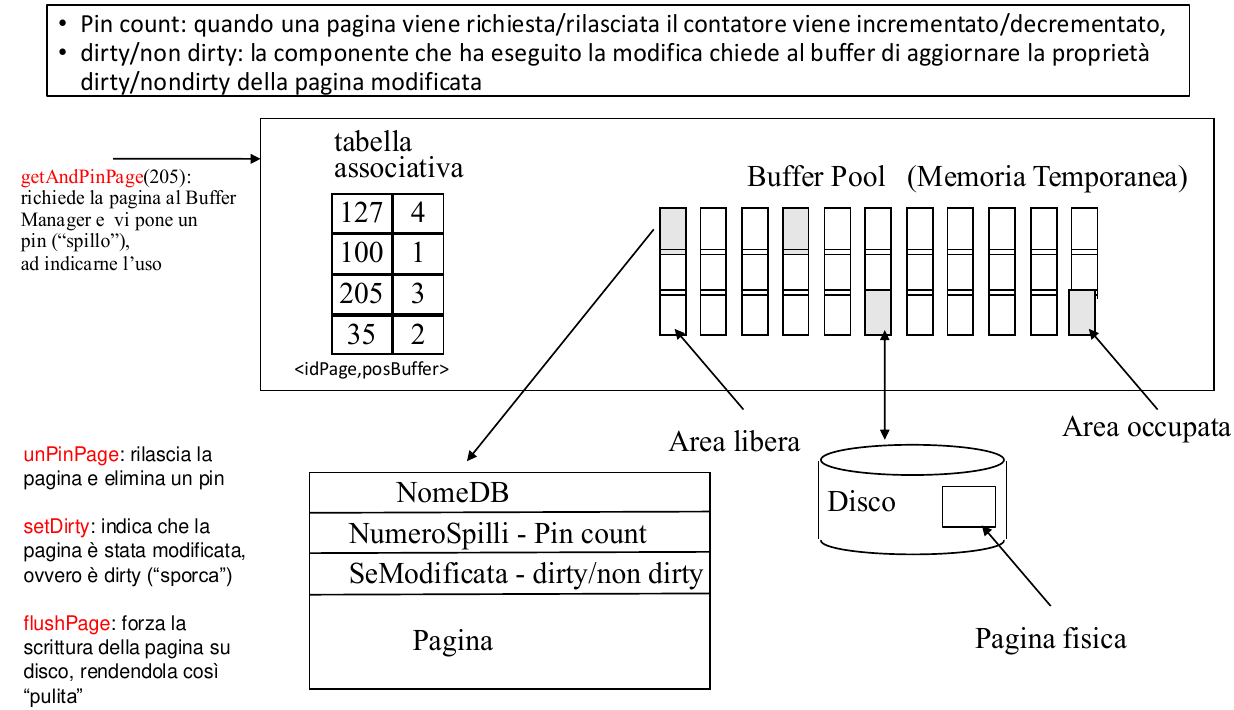
\includegraphics[scale=0.35]{gestore_buffer.png}
\end{center}

\subsubsection{Rimpiazzamento}
Nei sistemi operativi una comune politica adottata per decidere quale pagina rimpiazzare è la \textbf{LRU} (Least Recently Used), ovvero si rimpiazza la pagina che da più tempo non è in uso. Nei DBMS, non è sempre una buona scelta, in quanto per alcune query il pattern di accesso ai dati è noto, e può quindi essere utilizzato per operare con migliori prestazioni. L’\textbf{hit ratio}, ovvero la frazione di richieste che non provocano una operazione di I/O, indica sinteticamente quanto buona è una politica di rimpiazzamento.

\subsection{Strutture di memorizzazione}
Ci sono tre tipi di organizzazione per le strutture di memorizzazione:
\begin{itemize}
	\item \textbf{Seriali} o \textbf{sequenziali}
	\item Per \textbf{chiave}
	\item Per \textbf{attributi non chiave}
\end{itemize}
Per valutarli si presta attenzione a:
\begin{itemize}
	\item Occupazione di \textbf{memoria}
	\item \textbf{Costo} delle operazioni di \textit{ricerca}, \textit{modifica}, \textit{inserzione} e \textit{cancellazione}
\end{itemize}

\subsubsection{Seriale}
In questo tipo di organizzazione i dati sono memorizzati uno dopo l'altro nell'ordine in cui sono inseriti nel DB. È \textbf{semplice}, \textbf{economica} a livello di memoria ma \textbf{poco efficiente}. È l'organizzazione standard e va bene per pochi dati.

\subsubsection{Sequenziale}
A differenza di quella seriale, questa organizzazione \textbf{ordina} i dati sul valore di uno o più attributi. Questo garantisce velocità maggiore per ordinamento, raggruppamento e ricerca ma velocità minore per aggiornamento, cancellazione ed inserimento (va periodicamente riordinata la struttura).\\
La \textbf{ricerca} in un file di $b_i$ blocchi si compone di:
\begin{itemize}
	\item ricerca binaria nel file
	\item accesso al blocco
\end{itemize}
con un costo complessivo di $\log_2{b_i}+1$ per blocco.

\subsubsection{Chiave}
Questa organizzazione prevede due alternative: il metodo \textbf{procedurale} o \textbf{tabellare}.

\paragraph{Procedurale statico}
Questo approccio si basa sul file \textbf{hash}: al suo interno i record vengono allocati in una pagina il cui indirizzo dipende dal valore di chiave del record:
\begin{equation*}
	\text{key} \longrightarrow H(\text{key}) \longrightarrow \text{page address}
\end{equation*}
I parametri di questo metodo sono:
\begin{itemize}
	\item \textbf{Funzione} per la chiave (generalmente il resto della divisione intera)
	\item \textbf{Fattore di caricamento}, ovvero la frazione dello spazio fisico disponibile mediamente utilizzata.
	\item \textbf{Capacità} $c$ delle pagine
	\begin{equation}
		d = \frac{N}{M * c}
	\end{equation}
	Dove $N$ è il numero di tuple previste e $M$ il fattore di pagine. Il file potrà quindi prevedere un numero di blocchi $B$ pari al numero intero subito superiore a $d$.
	\item Metodo per la gestione di \textbf{overflow}: generalmente vengono usate liste linked
\end{itemize}

\begin{center}
	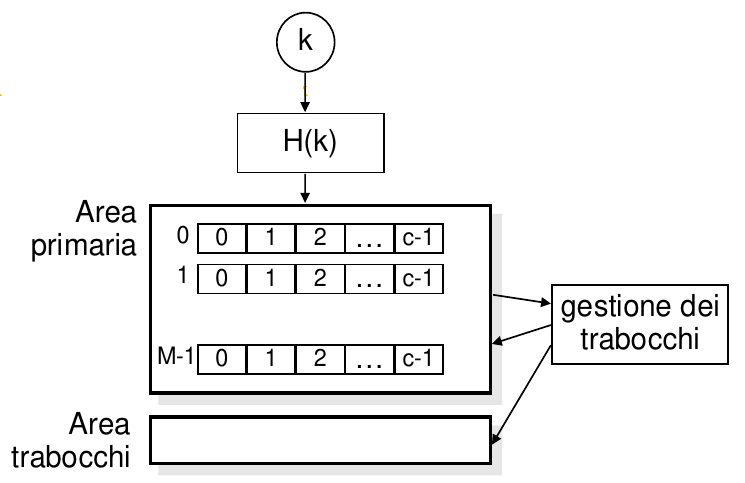
\includegraphics[scale=0.3]{procedurale.png}
\end{center}

Questo metodo è molto efficiente per \textbf{accesso puntuale} (uguaglianza di valori) ma non quando sono presenti intervalli o quando vengono usati attributi non chiave. Funziona solo con file la cui dimensione non varia molto nel tempo. Il \textbf{trade-off} principale riguarda il rapporto tra numero di blocchi e dimensione del DB:
\begin{itemize}
	\item Se è \textbf{piccolo} si hanno frequenti collisioni con overflow
	\item Se è \textbf{grande} si ha un fattore di riempimento basso
\end{itemize}
\newpage
\paragraph{Tabellare}
Il metodo tabellare sfrutta un \textbf{indice}, ovvero un insieme ordinato di coppie del tipo $(k, r(k))$, dove $k$ è un valore della chiave e $r(k)$ è un riferimento al record di chiave $k$. L'indice (che può anche essere \textbf{multiattributo}) viene gestito con un albero di tipo $\text{\textbf{B}}^\mathbf{+}$\textbf{-albero}.

\subparagraph{B-Tree}
Un B-tree di ordine $p$ deve soddisfare:
\begin{itemize}
	\item Ogni nodo interno ha la forma
	\begin{equation*}
		<P_1, <K_1, Pr_1>, P_2, <K_2, Pr_2>, \ldots, <K_{q-1}, Pr_{q-1} >, P_q > \qquad\qquad q \leq p
	\end{equation*}
	\begin{itemize}
		\item $P_i$ è un puntatore ad un altro nodo dell'albero (\textbf{tree pointer})
		\item $K_i$ è la chiave di ricerca
		\item $Pr_i$ è un puntatore ad un record il cui campo chiave di ricerca è uguale a $K_i$ o alla pagina che contiene tale record (\textbf{data pointer})
	\end{itemize}
	\item Per ogni nodo vale
	\begin{equation*}
		K_1 <K_2 < \ldots < K_{q-1}
	\end{equation*}
	\item Ogni nodo ha al più $p$ tree pointer
	\item Per tutti i valori $X$ della chiave di ricerca appartenenti al sottoalbero puntato da $P_i$ valgono
	\begin{align*}
		& K_{i-1} < X < K_i & 1 < i < q \\
		& X < K_i & i=1 \\
		& K_{i-1} < X & i=q
	\end{align*}
	\item La radice ha almeno due tree pointer a meno che non sia l'unico nodo
	\item Ogni nodo, esclusa la radice, ha almeno $\lceil \frac{p}{2} \rceil$ tree pointer. Un nodo con $q$ tree pointer ($q\leq p$) ha $q-1$ campi chiave di ricerca e $q-1$ data pointer
	\item Tutti i nodi foglia sono posti allo stesso livello. Hanno la stessa struttura degli altri tranne che tutti i loro tree pointer sono nulli
\end{itemize}
\begin{center}
	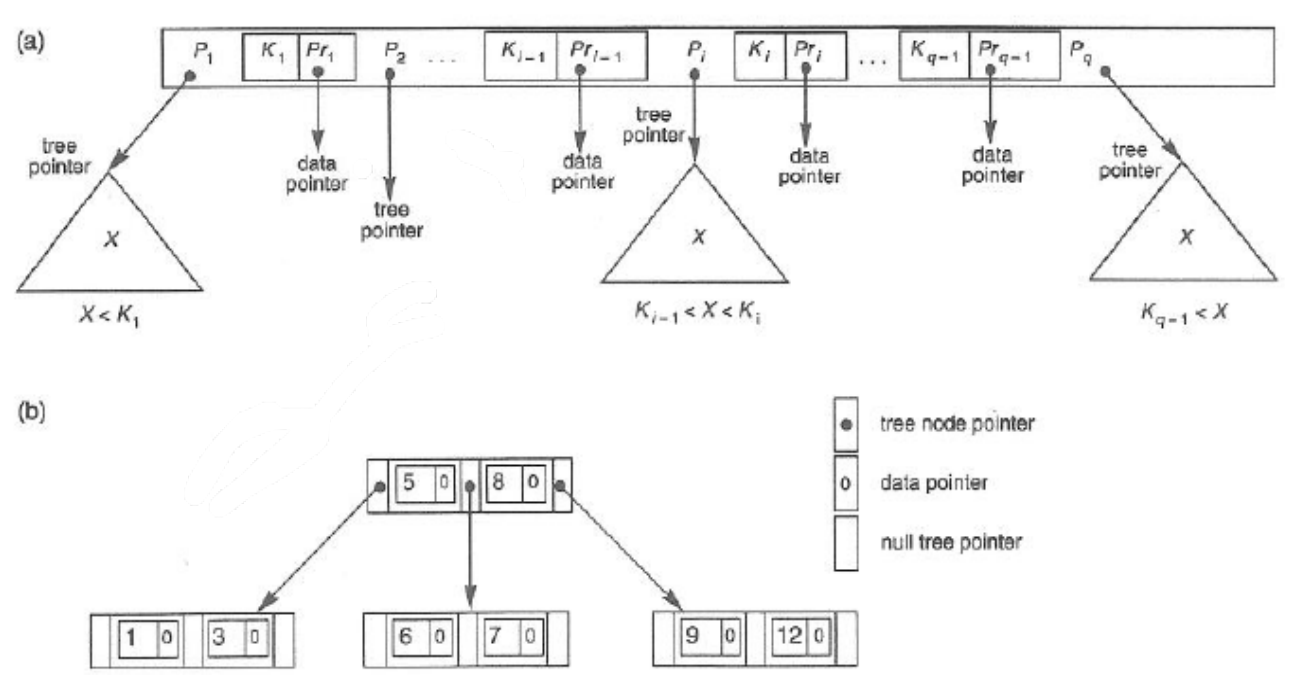
\includegraphics[scale=0.35]{btree.png}
\end{center}

\newpage
\subparagraph{$\text{\textbf{B}}^\mathbf{+}$-tree}
Un $\text{\textbf{B}}^\mathbf{+}$-tree è un B-tree in cui i data pointer sono memorizzati solo nei nodi foglia. La struttura dei nodi foglia quindi cambia come segue:
\begin{itemize}
	\item Se il campo di ricerca è un \textbf{campo chiave} i nodi foglia hanno per ogni valore del campo di ricerca una entry e un puntatore ad un record
	\item Se il campo di ricerca \textbf{non} è un campo chiave i puntatori indirizzano un blocco che contiene i puntatori a record dei file di dati
\end{itemize}
I nodi foglia di questo tipo di albero vengono generalmente messi in relazione e corrispondono al primo livello dell'indice mentre quelli interni agli altri livelli. Alcuni valori del campo di ricerca presenti nei nodi foglia sono ripetuti nei nodi interni per facilitare la ricerca.\\
La struttura dei \textbf{nodi interni} è la seguente:
\begin{itemize}
	\item Ogni nodo interno ha la forma
	\begin{equation*}
		<P_1, K_1, P_2, K_2, \ldots, P_{q-1}, K_{q-1}, P_q > \qquad\qquad q \leq p
	\end{equation*}
	dove ogni $P_i$ è un \textbf{tree pointer}
	\item Per ogni nodo interno vale
	\begin{equation*}
		K_1 < K_2 < \ldots K_{q-1}
	\end{equation*}
	\item Ogni nodo ha al più $p$ tree pointer
	\item Per tutti i valori $X$ della chiave di ricerca appartenenti al sottoalbero puntato da $P_i$ valgono
	\begin{align*}
	& X \leq K_i & i = 1\\
	& K_{i-1} < X \leq K_i & 1 < i < q \\
	& K_{i-1} < X & i=q
	\end{align*}
	\item Ogni nodo, esclusa la radice, ha almeno $\lceil \frac{p}{2} \rceil$ tree pointer. La radice ha almeno $2$ tree pointer se è un nodo interno
	\item Un nodo interno con $q$ tree pointer ($q \leq p$) ha $q-1$ campi di ricerca
\end{itemize}
\begin{center}
	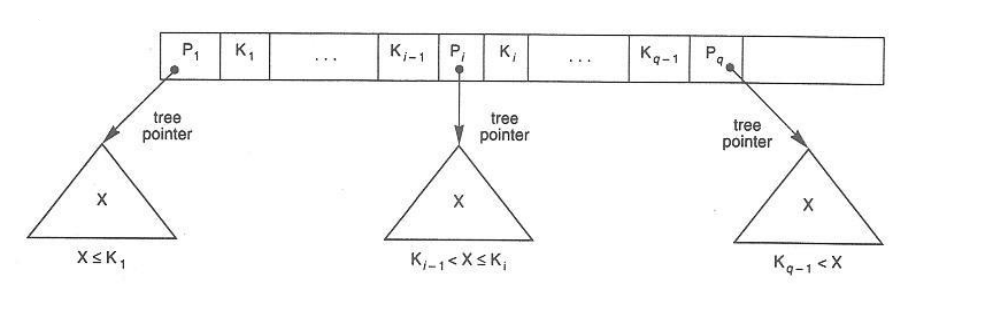
\includegraphics[scale=0.3]{binterni.png}
\end{center}

La struttura dei \textbf{nodi foglia} è la seguente:
\begin{itemize}
	\item Ogni nodo foglia è della forma
	\begin{equation*}
		<<K_1, Pr_1>, <K-2, Pr_2>, \ldots, <K_q, Pr_q>, P_{\text{next}}> \qquad q \leq p_{\text{leaf}}
	\end{equation*}
	\begin{itemize}
		\item $P_{next}$ è un \textbf{tree pointer}
		\item Ogni $Pr_i$ è un \textbf{data pointer} che punta al record con valore del campo di ricerca uguale a $K_i$ o ad un blocco contenente tale record o ad un blocco di puntatori ai record con
		valore del campo di ricerca uguale a $K_i$ , se il campo di ricerca non è una chiave
	\end{itemize}
	\item Per ogni nodo vale
	\begin{equation*}
		K_1 < K_2 < \ldots < K_q
	\end{equation*}
	\item Ogni nodo foglia ha almeno $\lceil \frac{p_{\text{leaf}}}{2} \rceil$ valori
	\item Tutti i nodi foglia sono dello stesso livello
\end{itemize}

\begin{center}
	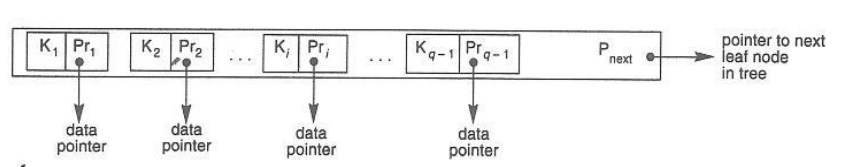
\includegraphics[scale=0.3]{bfoglia.png}
\end{center}

\subparagraph{Tipi di indice}
Gli indici ad albero esistono di due tipi:
\begin{itemize}
	\item \textbf{Statici}: la struttura viene creata sulla base dei dati presenti nel DB e non viene modificata
	\item \textbf{Dinamici}: la struttura albero viene aggiornata ad ogni operazione
\end{itemize}

\subsubsection{Indici}
\begin{definition}[Indice]
	Un indice è una struttura che contiene informazioni sulla posizione di memorizzazione delle tuple sulla base del valore del campo chiave.
\end{definition}
Gli indici  si distinguono tra:
\begin{itemize}
	\item \textbf{Primario}: la chiave di ordinamento del file sequenziale coincide con la chiave di ricerca dell'indice. È un file \textbf{ordinato} in cui i record sono di lunghezza fissa e sono costituiti da:
	\begin{itemize}
		\item Un campo dello stesso tipo della \textbf{chiave primaria}
		\item Un \textbf{puntatore al blocco del disco}
	\end{itemize}
	Esiste un record $<K(i), RID(i)>$ per ogni blocco.
	\item \textbf{Secondario}: la chiave di ordinamento e quella di ricerca sono diverse. Può essere definito:
	\begin{itemize}
		\item Su un campo non chiave che è una chiave candidata a valori univoci
		\item Su un campo non chiave con valori duplicati
	\end{itemize}
	I record sono composti da:
	\begin{itemize}
		\item Campo di \textbf{indicizzazione}: dello stesso tipo del campo che non viene usato per ordinare il file
		\item \textbf{Puntatore} al \textbf{blocco} o al \textbf{record} (RID)
	\end{itemize}
\end{itemize}
Un indice può essere definito su un insieme di attributi $A_1, A_2, \ldots, A_n$ e in questo caso contiene un record per ogni combinazione di valori degli attributi. Rende più efficiente l'interrogazione di specifiche combinazioni di valori.

\subsubsection{Ordinamento}
L'ordinamento nei DB è importante per le operazioni ORDER BY e per le operazioni relazionali JOIN, SELECT e GROUP BY. Può anche servire per eliminare i duplicati nella DISTINCT.\\
L'algoritmo più utilizzato è \textbf{Z-Way Sort Merge} e si compone di due fasi. Assumendo di avere $NP$ pagine e $NB < NP$ buffer in memoria centrale:
\begin{enumerate}
	\item \textbf{Sort interno}: si leggono una alla volta le pagine del file; i record di ogni pagina vengono ordinati facendo uso di un algoritmo di sort interno (e.g. Quicksort). Ogni pagina così ordinata, detta anche \textbf{run}, viene scritta su disco in un file temporaneo
	\item \textbf{Merge}: operando uno o più passi di fusione, le run vengono fuse, fino a produrne una unica
\end{enumerate}

\begin{example}[Caso base]
	Assumiamo di avere un caso a $2$ vie con $NB = 3$ buffer in memoria centrale.
	\begin{center}
		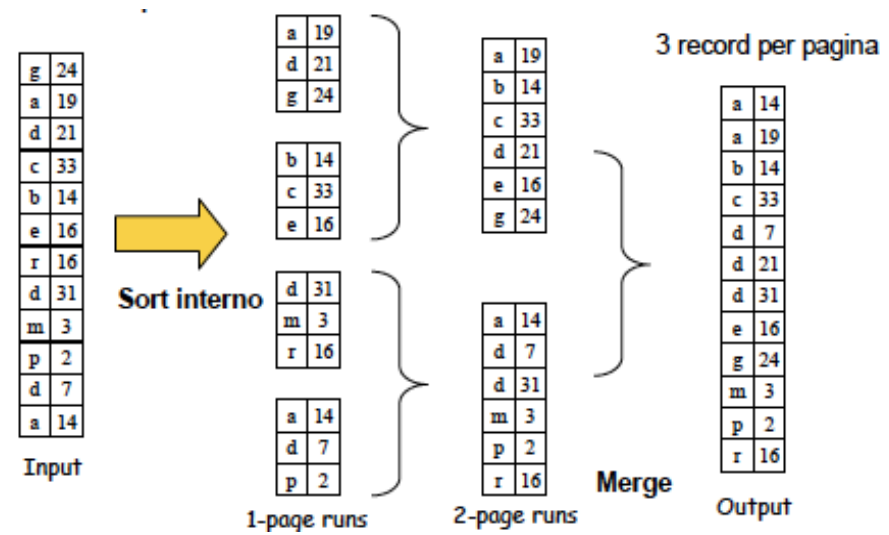
\includegraphics[scale=0.3]{zsort.png}
	\end{center}
\end{example}

\paragraph{Complessità}
Considerando che nel passo di sort interno, avendo a disposizione $NB$ buffer, si possono ordinare $NP$ pagine alla volta (anziché una sola), porta ad un costo di $2 \cdot NP \cdot (\lceil \log_2(\frac{NP}{NB})\rceil + 1)$.

\subsection{Operatori relazionali}
\subsubsection{Proiezione}
\begin{lstlisting}[language=SQL]
	SELECT DISTINCT Provincia
	FROM Studenti R
\end{lstlisting}
Uno degli approcci per la realizzazione della proiezione con \textbf{DISTINCT} è tramite l'\textbf{ordinamento}:
\begin{enumerate}
	\item Si legge la relazione $R$ e si scrive in un'altra $T$ solo i valori interessati dalla SELECT
	\item Si ordina $T$ su tutti gli attributi
	\item Si eliminano i duplicati
\end{enumerate}

\subsubsection{Restrizione}
\begin{lstlisting}[language=SQL]
	SELECT *
	FROM Studenti R
	WHERE R.Provincia = 'PI'
\end{lstlisting}
Vediamo i due approcci:
\begin{itemize}
	\item Con \textbf{indice}: usando il $\text{\textbf{B}}^+$\textbf{-albero} si ha $\text{Costo Accesso Indice} + \text{Costo Accesso Dati}$
	\item \textbf{Senza indice} e con dati disordinati: $N_{\text{pag}}(R)$
\end{itemize}

\subsubsection{Aggregazione}
Abbiamo due casi:
\begin{itemize}
	\item \textbf{Senza} GROUP BY: si visitano i dati e si calcolano le funzioni di aggregazione
	\begin{lstlisting}[language=SQL]
		SELECT COUNT(*) FROM Persone
	\end{lstlisting}
	\item \textbf{Con} GROUP BY: si ordinano i dati sugli attributi del GROUP BY, poi li si visitano e si
	calcolano le funzioni di aggregazione per ogni gruppo
	\begin{lstlisting}[language=SQL]
		SELECT Cognome, COUNT(Cognome)
		FROM Persone
		GROUP BY Cognome
	\end{lstlisting}
\end{itemize}

\subsubsection{Giunzione}
\begin{lstlisting}[language=SQL]
	SELECT *
	FROM Studenti S, Esami E
	WHERE S.Matricola=E.Matricola
\end{lstlisting}
Anche se logicamente il Join è commutativo, dal punto di vista fisico vi è una differenze nelle prestazioni tra operando sinistro (o esterno) e destro (interno).

\paragraph{Nested Loop}
L'approccio basilare è quello \textbf{Nested Loops}, ovvero
\begin{lstlisting}[language=SQL, mathescape]
	foreach record in R do
		foreach record in S do
			if $r_j = s_j$ then
				add $<r,s>$ to risultato
\end{lstlisting}
In questo approccio il costo computazionale varia in base alla scelta della relazione esterna ed è
\begin{equation}
	N_{\text{pag}}(R) + N_{\text{rec}}(R) \cdot N_{\text{pag}}(S) \approx N_{\text{pag}}(R) \cdot \frac{N_{\text{rec}}(R)}{N_{\text{pag}}(R)} \cdot N_{\text{pag}}(S)
\end{equation}
Bisognerà quindi scegliere come relazione esterna quella con record più lunghi e/o grandi.
\begin{equation*}
	\frac{N_{\text{rec}}(R)}{N_{\text{pag}}(R)} < \frac{N_{\text{rec}}(S)}{N_{\text{pag}}(S)}
\end{equation*}

\begin{note}
	L'ordine con cui vengono generate le tuple coincide con l'ordine della relazione esterna. In caso di ORDER BY è quindi importante la scelta della relazione esterna anche da questo punto di vista.
\end{note}

\subparagraph{Page}
Una variante molto comune del Nested Loop è quella a \textbf{pagine}. Questa rinuncia a preservare l'ordine della relazione esterna in quanto esegue il join di tutte le tuple già presenti in memoria prima di richiedere nuove pagine. Il costo è ora di $NP(R)+NP(R) \cdot NP(S)$ operazioni di input/output.
\begin{lstlisting}[language=SQL, mathescape]
	Per ogni pagina $p_R$ di R:
		{ Per ogni pagina $p_S$ in S:
			{ esegui il join di tutte le tuple in $p_R$ e $p_S$ } }
\end{lstlisting}
\subparagraph{Index}
Una variante del Nested Loop prevede che, data una tupla della relazione esterna $R$, la scansione completa della relazione interna $S$ può essere sostituita da una scansione basata su un indice costruito sugli attributi di join di $S$, secondo il seguente schema:
\begin{center}
	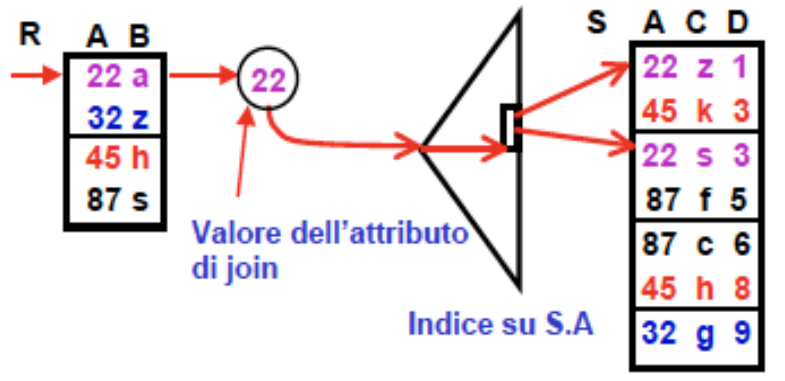
\includegraphics[scale=0.3]{indexnestedloop.png}
\end{center}
\begin{lstlisting}[language=SQL, mathescape]
	foreach record r in R do
		foreach record s in get-through-index($IS_j=r_i$) do
			add $<r, s>$ to risultato
\end{lstlisting}
L’accesso alla relazione interna mediante indice porta in generale a ridurre di molto i costi di esecuzione del Nested Loops Join.
\subparagraph{Sort-Merge}
L'approccio di Sort-Merge è applicabile quando entrambi gli insiemi di tuple sono \textbf{ordinati} sugli attributi di join. Questo è possibile per $R(S)$ se:
\begin{itemize}
	\item È \textbf{fisicamente ordinata} sugli attributi di join
	\item Esiste un \textbf{indice} sugli attributi di join di $R(S)$
\end{itemize}
La logica dell’algoritmo (senza considerare il tempo per il sort) sfrutta il fatto che entrambi gli input sono ordinati per evitare di fare inutili confronti, il che fa sì che il numero di letture sia dell’ordine di:
\begin{equation*}
	N_{\text{pag}}(R) + N_{\text{pag}}(S)
\end{equation*}
se si accede sequenzialmente alle due relazioni.

\begin{lstlisting}[language=SQL, mathescape]
	r = first(R); s = first(S);
	while r in R and s in S do
		if $r_i = s_j$
			avanza r e s fino a che $r_i$ e $s_j$ sono uguali,
			aggiungendo ciascun $<r, s>$ al risultato
		else if $r_i < s_j$ avanza r dentro R
		else if $r_i > s_j$ avanza s dentro S
\end{lstlisting}

\subsection{Piani d'accesso}
Un piano di accesso è un’\textbf{espressione algebrica} in cui gli operatori logici sono sostituiti da operatori fisici.

\begin{example}[Piano d'accesso]
	Data la seguente query
	\begin{lstlisting}[language=SQL]
		SELECT Nome
		FROM Studenti S, Esami E
		WHERE S.Matricola=E.Matricola AND
		Provincia='PI' AND Voto>25
	\end{lstlisting}
	vediamo l'albero logico e il suo piano d'accesso:
	\begin{figure}[!h]
		\centering
		\begin{minipage}{.45\textwidth}
			\centering
			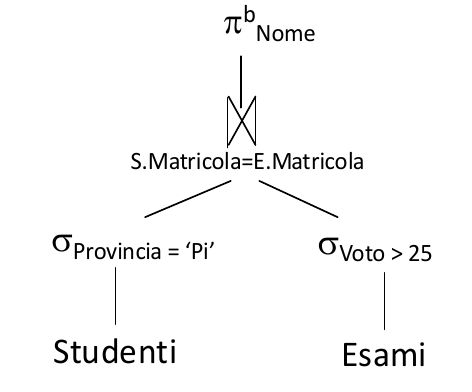
\includegraphics[scale=0.3]{esempiopianilogico.png}
			\captionof{figure}{Albero logico}
		\end{minipage}
		\begin{minipage}{.45\textwidth}
			\centering
			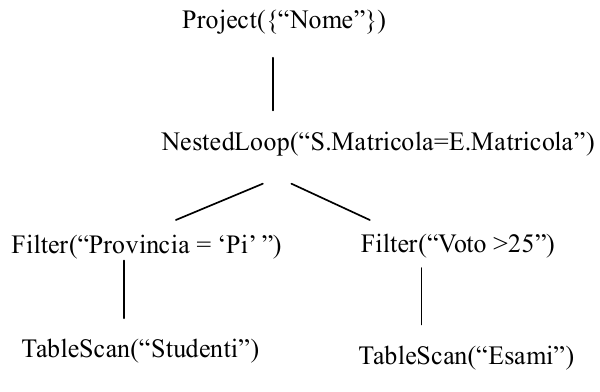
\includegraphics[scale=0.3]{esempiopianoaccesso.png}
			\captionof{figure}{Piano d'accesso}
		\end{minipage}
	\end{figure}
\end{example}
\subsubsection{Ottimizzatore}
L'ottimizzazione delle interrogazioni è fondamentale nei DBMS. L'ottimizzazore ha come obiettivo quello di scegliere il piano con costo minimo usando le statistiche presenti nel catalogo. Si divide nelle seguenti fasi:
\begin{enumerate}
	\item \textbf{Analisi e semplificazione}: prende in input il \textbf{comando} e il \textbf{catalogo}. Verifica la correttezza del comando ed esegue normalizzazione e semplificazione della condizione. Passa al successivo l'\textbf{albero logico}.
	\begin{center}
		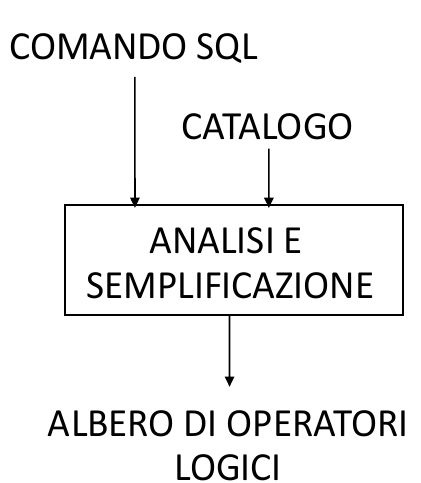
\includegraphics[scale=0.2]{ottimiz1}
	\end{center}
	\item \textbf{Trasformazione}: prende in ingresso l'albero di operatori logici ed esegue trasformazioni con regole di equivalenza, restituendone un altro
	\begin{center}
		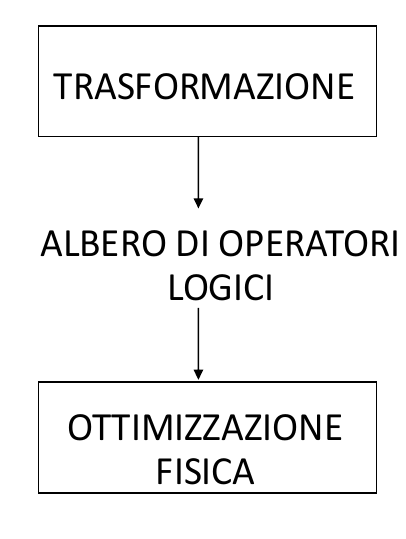
\includegraphics[scale=0.2]{ottimiz2}
	\end{center}
	\item \textbf{Ottimizzazione fisica}: dato l'albero logico si fanno e scelte degli algoritmi da eseguire, evitando i peggiori, restituendo un \textbf{piano di accesso}
	\begin{center}
		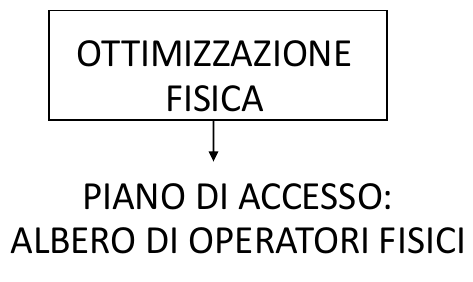
\includegraphics[scale=0.2]{ottimiz3}
	\end{center}
	\item \textbf{Esecuzione}: esegue il piano d'accesso e restituisce il risultato
	\begin{center}
		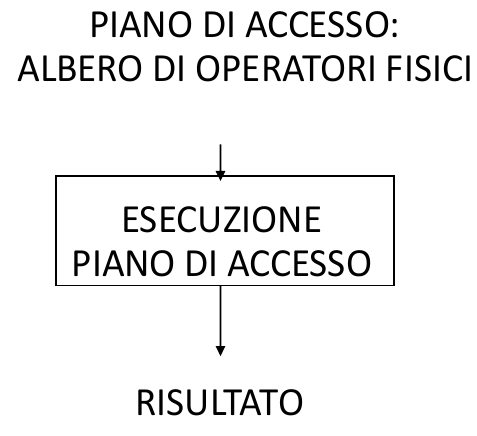
\includegraphics[scale=0.2]{ottimiz4}
	\end{center}
\end{enumerate}
\subsubsection{Operatori fisici}
Un operatore logico può essere realizzato con algoritmi diversi codificati in operatori fisici. Ognuno di questi è un \textbf{iteratore}, un oggetto dotato dei seguenti metodi:
\begin{itemize}
	\item \textbf{open}: inizializza lo stato dell’operatore, alloca buffer per gli input e l’output, richiama ricorsivamente open sugli operatori figli. Viene anche usato per passare argomenti (e.g. la condizione che un operatore Filter deve applicare)
	\item \textbf{next}: richiede un’altra tupla del risultato dell’operatore. L’implementazione include \textit{next} sugli operatori figli e codice specifico dell’operatore
	\item \textbf{close}: termina l’esecuzione dell’operatore, con conseguente rilascio delle risorse allocate
	\item \textbf{isDone}: indica se vi sono ancora valori da leggere, in genere è booleano
	\item \textbf{reset}
\end{itemize}

\bgroup
\def\arraystretch{1.5}
\begin{table}[!h]
	\centering
	\begin{tabular}{|M{100pt}|M{300pt}|}
		\hline
		\textbf{Operatore logico} & \textbf{Operatore fisico} \\
		\hline
		& $\text{TableScan(R)}$ \linebreak per la scansione di $R$ \\ \cline{2-2}
		$R$& $\text{IndexScan}(R, Idx)$ \linebreak per la scansione di $R$ con indice $Idx$ \\ \cline{2-2}
		& $\text{SortSca}(R, \{A_i\})$ \linebreak per la scansione di $R$ ordinata sugli $\{A_i\}$\\ \cline{2-2}
		\hline
		\multirowcell{2}{$\pi_{\{A_i\}}$} & $\text{Project}(O, \{A_i\})$\linebreak per la proiezione dei record di $O$ senza eliminazione dei duplicati \\ \cline{2-2}
		& $\text{Distinct}(O)$ \linebreak per eliminare i duplicati dei record ordinati di $O$ \\
		\hline
		\multirowcell{2}{$\sigma_{\psi}$} & $\text{Filter}(O, \psi)$ \linebreak per la restrizione senza indici dei record di $O$ \\ \cline{2-2}
		& $\text{IndexFilter}(R, Idx, \psi)$ \linebreak per la restrizione con indice dei record di $R$ \\
		\hline
		$\tau_{\{A_i\}}$ & $\text{Sort}(O,\{A_i\})$ \linebreak per ordinare i record di $O$ sugli $\{A_i\}$, per valori crescenti \\
		\hline
		$\prescript{}{\{A_i\}}{\gamma}_{\{f_i\}}$ & $\text{GroupBy}(O, \{A_i\}, \{f_i\})$ \linebreak per raggruppare i record di $O$ sugli $\{A_i\}$ usando le funzioni di aggregazione in $\{f_i\}$.
		\begin{itemize}
			\item Nell'insieme $\{f_i\}$ vi sono le funzioni di aggregazione presenti nella SELECT e nella HAVING
			\item L'operatore restituisce record con attributi gli $\{A_i\}$ e le funzioni in $\{f_i\}$
			\item I record di $O$ sono ordinati sugli $\{A_i\}$
		\end{itemize} \\
		\hline
		& $\text{NestedLoop}(O_E, O_I, \psi_J)$ \linebreak per la giunzione con il nested loop e $\psi_J$ la condizione di giunzione \\ \cline{2-2}
		& $\text{PageNestedLoop}(O_E, O_I, \psi_J)$ \linebreak per la giunzione con il page nested loop \\ \cline{2-2}
		\multirowcell{4}{$\overset{\Join}{\psi_J}$} & $\text{IndexNestedLoop}(O_E, O_I, \psi_J)$ \linebreak per la giunzione con index nested loop. $O_I$ è un $\text{IndexFilter}(R, Idx, \underline{\psi_J})$ oppure $\text{Filter}(O, \psi')$ con $O$ un $\text{IndexFilter}(R, Idx, \underline{\psi_J})$. Per ogni record $r$ di $O_E$, la condizione $\psi_J$ dell'\textit{IndexFilter} è quella di giunzione con gli attributi di $O_E$ sostituiti dai valori in $r$ \\ \cline{2-2}
		& $\text{SortMerge}(O_E, O_I, \psi_J)$ \linebreak per la giunzione con il sort-merge, con i record di $O_E$ e $O_I$ ordinati sugli attributi di giunzione \\
		\hline
	\end{tabular}
\end{table}
\egroup
\newpage
\subsection{Transazioni}
Una funzionalità essenziale di un DBMS è la \textbf{protezione} dei dati da malfunzionamenti e da interferenze dovute all’accesso contemporaneo ai dati. La \textbf{transazione} per il programmatore è un programma sequenziale costituito da operazioni che il sistema deve eseguire garantendo \textbf{atomicità}, \textbf{serializzabilità} e \textbf{persistenza}. 

\subsubsection{Gestione delle transazioni}
\begin{definition}[Transazione]
	Una transazione è una sequenza di azioni di lettura e scrittura in memoria permanente e di elaborazioni di dati in memoria temporanea, con le seguenti proprietà:
	\begin{itemize}
		\item \textbf{Atomicità}: le transazioni che terminano prematuramente (aborted) non lasciano effetti sulla BD (eventuali effetti sono annullati)
		\item \textbf{Serializzabilità}: nel caso di esecuzioni concorrenti di più transazioni l'effetto complessivo è quello di un'esecuzione seriale
		\item \textbf{Persistenza}: le modifiche su una base di dati di una transazione terminata normalmente sono permanenti (non alterabili da malfunzionamenti)
	\end{itemize}
\end{definition}
\noindent Inoltre una transazione deve anche rispettare le proprietà \textbf{ACID}:
\begin{itemize}
	\item \textbf{Atomicità}: la transazione deve essere completamente eseguita o annullata
	\item \textbf{Consistenza}: la transazione deve lasciare il DB in uno stato consistente (eventuali vincoli non devono essere violati)
	\item \textbf{Isolamento}: l'esecuzione di una transazione deve essere indipendente dalle altre
	\item \textbf{Durability}: l'effetto di una transazione conclusa non deve essere perso
\end{itemize}
Sintatticamente una transazione è situata tra i comandi \textbf{begin transaction} ed \textbf{end transaction} e all'interno possono comparire \textbf{rollback work} o \textbf{commit work}.
\begin{lstlisting}[language=SQL]
	begin transaction
	update SalariImpiegati
	set conto=conto-10
	where (CodiceImpiegato = 123)
	if conto >0 commit work;
	else rollback work
\end{lstlisting}

Per aumentare le prestazioni i DBMS usano un \textbf{buffer temporaneo} di informazioni in memoria principale che viene periodicamente scritto su memoria secondaria.
\begin{center}
	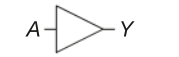
\includegraphics[scale=0.3]{buffer}
\end{center}

Al DBMS importano solamente le operazioni di scrittura e lettura. Un dato può essere un \textbf{record}, un \textbf{campo} o una \textbf{pagina}. Analizziamo le operazioni:
\begin{itemize}
	\item \textbf{Lettura} $r_i[x]$: comporta la lettura di un dato nel buffer se non già presente
	\item \textbf{Scrittura} $w_i[»]$: comporta l'\textbf{eventuale} lettura del buffer di un dato e la sua modifica nel buffer ma non necessariamente la scrittura su memoria permanente. Ergo per cui si potrebbe perdere l'effetto dell'operazione in caso di malfunzionamento
\end{itemize}
\paragraph{Malfunzionamento}
Esistono tre tipi di malfunzionamento:
\begin{itemize}
	\item \textbf{Fallimenti di transazione}: non comportano la perdita di dati
	\item \textbf{Fallimenti di sistema}: comportano la perdita di dati in \textbf{memoria temporanea} ma non in quella persistente
	\item \textbf{Disastri}: comportano la perdita di dati in \textbf{memoria persistente}
\end{itemize}
\subsubsection{Gestione dell'affidabilità}
Il gestore dell'affidabilità verifica che siano garantite le proprietà di  \textbf{atomicità} e \textbf{persistenza}. È il responsabile dei comandi \textit{commit}, \textit{rollback} e \textit{begin transaction} oltre che dei ripristini di sistema dopo malfunzionamenti:
\begin{itemize}
	\item \textbf{Software}, ripresa a caldo
	\item \textbf{Hardware}, ripresa a freddo
\end{itemize}
\paragraph{Logging}
Il gestore dell'affidabilità tiene traccia delle operazioni svolte in un file di \textbf{LOG}. Questo si presenta come un file \textbf{sequenziale} suddiviso in \textbf{record}, che possono essere:
\begin{itemize}
	\item Di \textbf{transazione}: tengono traccia delle operazioni svolte da ciascuna transizione sul DBMS. Per ogni transazione abbiamo:
	\begin{itemize}
		\item \textbf{Begin} (B)
		\item \textbf{Insert} (I)
		\item \textbf{Delete} (D)
		\item \textbf{Update} (U)
		\item \textbf{Commit} (C) o \textbf{Abort} (A)
	\end{itemize}
	\item Di \textbf{sistema}: tengono traccia delle operazioni di sistema quali \textbf{dump} e \textbf{checkpoint}
\end{itemize}
\subparagraph{Undo e Redo}
I record dei log di una transazione ci permettono di disfare e rifare le operazioni effettuate su una BD. Data una transazione $T$ su un oggetto $O$, dove $BS$ è before state e $AS$ è after state:
\begin{itemize}
	\item \textbf{UNDO}: ricopia in $O$ il valore $BS$
	\item \textbf{REDO}: ricopia in $O$ il valore $AS$
\end{itemize} 
\subparagraph{DUMP}
L'operazione di dump produce una copia (in una memoria stabile) completa della BD effettuata in \textbf{mutua esclusione} con tutte le altre transazioni quando il sistema non è operativo. Al termine del backup viene scritto nel \textit{LOG} un record di dump che ne segnala l'avvenimento.

\subparagraph{Regole di scrittura}
Esistono due regole principali per la scrittura nel file di LOG:
\begin{itemize}
	\item \textbf{Write Ahead Log}: la parte $BS$ di ogni record viene scritta prima che la corrispondente operazione venga eseguita
	\item \textbf{Commit Precedence}: la parte $AS$ di ogni record viene scritta prima di effettuare il commit della transazione
\end{itemize}
\begin{center}
	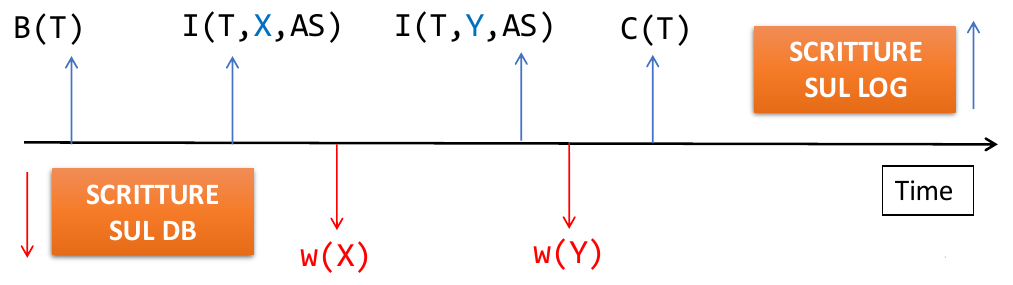
\includegraphics[scale=0.3]	{log}
\end{center}
\subparagraph{Checkpoint}
Al momento del ripristino, solo gli aggiornamenti più recenti nel log potrebbero non essere ancora nella BD. Per essere certi di quali sono state eseguite o meno, periodicamente si fa un Checkpoint (CKP):
\begin{enumerate}
	\item SI scrive sul giornale una marca d'inizio del checkpoint con le transazioni attive
	\begin{equation*}
		(\text{BeginCkp}, \{T_1, \ldots, T_n\})
	\end{equation*}
	\item In parallelo alle normali transazioni il gestore riporta sul disco tutte le pagine modificate
	\item Si scrive la marca \textbf{EndCkp} che certifica che tutte le operazioni prima di BeginCkp sono sul disco (quelle tra l'inizio e la fine, forse si o no)
\end{enumerate}
\paragraph{Algoritmi}
Gli algoritmi si differenziano a seconda del modo in cui si trattano le scritture sulla BD e la terminazione delle transazioni:
\begin{itemize}
	\item \textbf{Disfare-Rifare}
	\item \textbf{Disfare-NonRifare}
	\item \textbf{NonDisfare-Rifare}
	\item \textbf{NonDisfare-NonRifare}
\end{itemize}
\subparagraph{Disfare-Rifare}
Per \textbf{disfare} l'algoritmo usa la politica della \textbf{modifica libera}: le modifiche possono essere portate nella BD stabile prima che la transazione $T$ termini. Per poterla applicare è necessario usare la \textbf{WAL}: se la nuova versione di una pagina rimpiazza la vecchia sulla BD stabile prima che la transazione $T$ abbia raggiunto il punto di Commit, allora la vecchia versione della pagina deve essere portata prima sul giornale in modo permanente.\\
Per \textbf{rifare}, la terminazione viene gestita con la politica del \textbf{commit libero}: una transazione $T$ può essere considerata terminata normalmente prima che tutte le modifiche vengano riportate nella BD stabile, altrimenti si applica la \textbf{commit rule} e bisogna rifare.\\
Per quanto riguarda i malfunzionamenti questo algoritmo si comporta come segue:
\begin{itemize}
	\item Fallimenti di \textbf{transazioni}: si scrive nel giornale $(T, \text{abort})$ e si applica \textbf{disfare}
	\item Fallimenti di \textbf{sistema}: la BD viene ripristinata con \textbf{Restart} a partire dallo stato al Ckp: le $T$ non terminate vengono disfatte e quelle terminate rifatte
	\item \textbf{Disastri}: si riporta in linea la copia più recente della BD e la si aggiorna facendo le modifiche delle $T$ terminate normalmente (\textbf{ripresa a freddo})
\end{itemize}
La \textbf{ripresa a caldo} invece prevede:
\begin{enumerate}
	\item Trovare l'ultimo checkpoint
	\item Costruire gli insiemi \textbf{UNDO} e \textbf{REDO} delle transazioni
	\item Eseguire tutte le operazioni di UNDO
	\item Eseguire tutte le operazioni di REDO
\end{enumerate}
In questo modo si garantisce \textbf{atomicità} e \textbf{persistenza} delle transazioni.
\begin{center}
	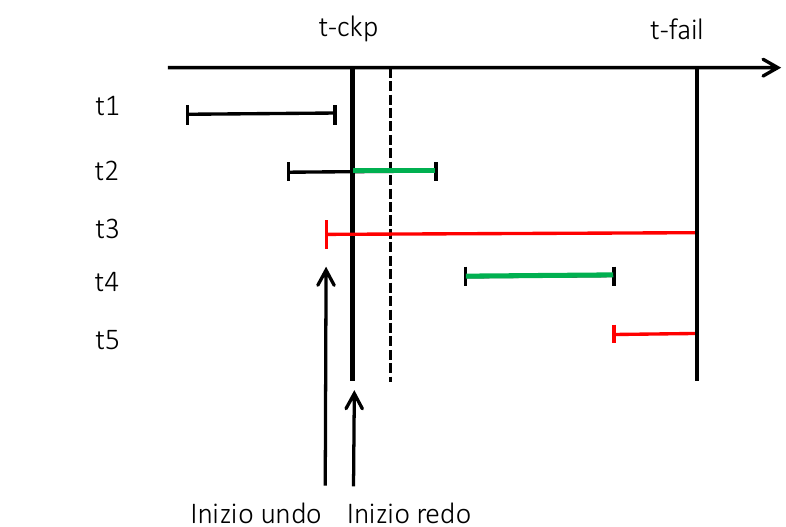
\includegraphics[scale=0.25]{ripartenzacaldo}
\end{center}
\subsubsection{Gestione della concorrenza}
L’esecuzione concorrente di transazioni è essenziale per un buon funzionamento del DBMS, che deve però garantire che
avvenga senza interferenze in caso di accessi agli stessi dati.

\begin{definition}[Serialità]
	Un’esecuzione di un insieme di transazioni $\{T_1, \ldots, T_n\}$ si dice seriale se, per ogni coppia di transazioni $T_i$ e $T_j$, tutte le operazioni di $T_i$ vengono eseguite prima di qualsiasi operazione $T_j$ o viceversa.
\end{definition}

\begin{definition}[Serializzabilità]
	Un’esecuzione di un insieme di transazioni si dice serializzabile se produce lo stesso effetto sulla base di dati di quello
	ottenibile eseguendo serialmente, in un qualche ordine, le sole transazioni terminate normalmente.
\end{definition}

Uno schedule $S=\{T_1, T_2, \ldots, T_n\}$ si dice \textbf{seriale} se le azioni di ciascuna transazione appaiono in sequenza, senza essere frammentate da azioni di altre. È ottenibile se:
\begin{itemize}
	\item Le transazioni sono eseguite uno alla volta (irrealistico)
	\item Le transazioni sono completamente \textbf{indipendenti} (improbabile)
\end{itemize}
\paragraph{Problematiche} Le problematiche principali della concorrenza sono:
\begin{itemize}
	\item \textbf{Perdita di aggiornamento}
	\begin{center}
		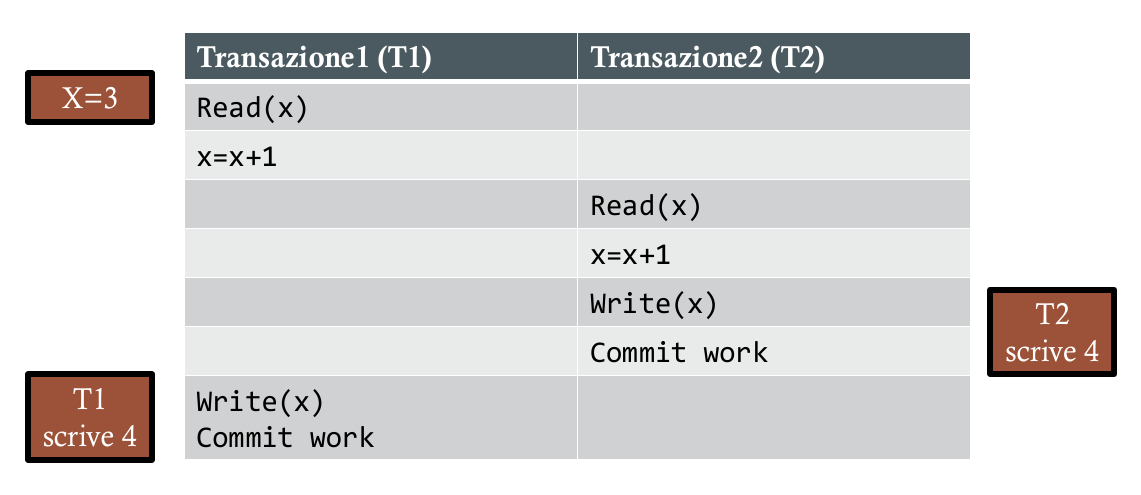
\includegraphics[scale=0.25]{perditaagg.png}
	\end{center}
	\item \textbf{Lettura sporca} o \textbf{impropria}
	\begin{center}
		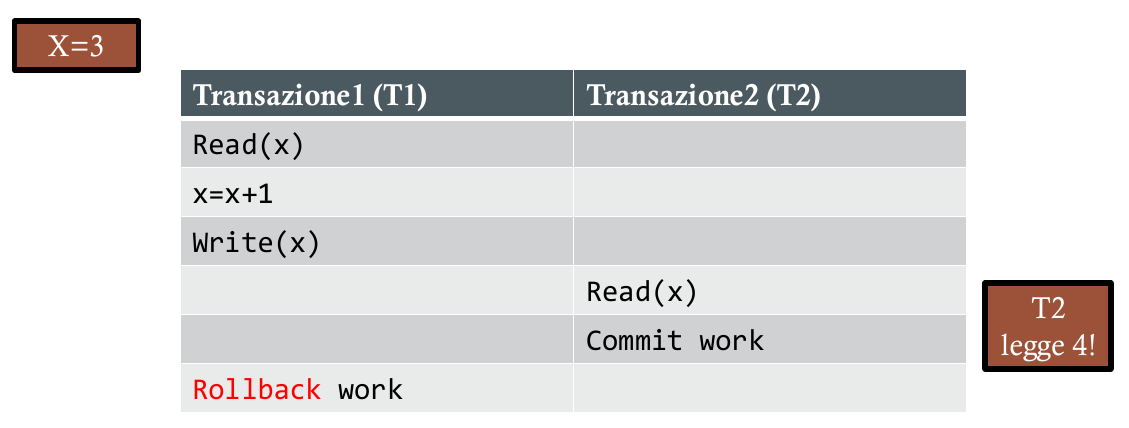
\includegraphics[scale=0.25]{letturasporca.png}
	\end{center}
	\item Letture \textbf{inconsistenti} o \textbf{non riproducibili}
	\begin{center}
		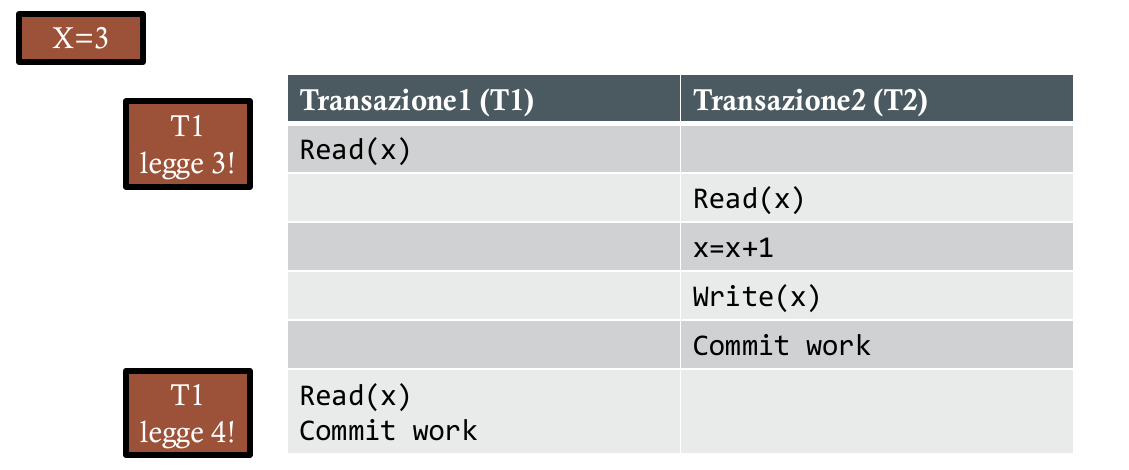
\includegraphics[scale=0.25]{lettureinconsistenti.png}
	\end{center}
\end{itemize}

\paragraph{Controllo della concorrenza}
Per gestire questi problemi il DBMS sfrutta la proprietà di \textbf{isolamento}, facendo si che un insieme di transazioni concorrenti siano serializzabili. Utilizza delle tecniche di controllo che si dividono in due classi:
\begin{itemize}
	\item Protocolli \textbf{pessimistici} o conservativi: tendono a ritardare l’esecuzione di	transazioni che potrebbero generare conflitti, e quindi anomalie, rispetto alla transazione corrente. Le tecniche principali sono:
	\begin{itemize}
		\item Metodi basati su \textbf{lock}
		\item Metodi basati su \textbf{timestamp}
	\end{itemize}
	\item Protocolli \textbf{ottimistici}: permettono l’esecuzione sovrapposta e non sincronizzata di transazioni ed effettuano un controllo sui possibili conflitti	generati solo dopo il commit. 
\end{itemize}

\subparagraph{Protocolli ottimistici}
Ogni transazione effettua liberamente le proprie operazioni secondo l’ordine temporale con cui le operazioni stesse sono generate. Al commit, viene effettuato un controllo per stabilire se sono stati riscontrarti eventuali conflitti, e nel caso, viene effettuato il rollback delle azioni delle transazioni e la relativa riesecuzione. \\
In generale, un protocollo di controllo di concorrenza ottimistico è basato su 3 fasi:
\begin{enumerate}
	\item \textbf{Lettura}: ogni transazione legge i valori degli oggetti della BD su cui deve operare e li copia in variabili locali dove sono effettuati eventuali aggiornamenti
	\item \textbf{Validazione}: vengono effettuati dei controlli sulla serializzabilità nel caso che gli aggiornamenti locali delle transazioni dovessero essere propagati sulla base di dati
	\item \textbf{Scrittura}: gli aggiornamenti delle transazioni che hanno superato la fase di validazione sono propagati definitivamente sugli oggetti della BD
\end{enumerate}

\subparagraph{Protocolli pessimistici con Lock}
Il lock è un meccanismo che blocca l'accesso ad altre transazioni (che vengono messe in coda) ai dati ai quali una transazione accede. Può essere:
\begin{itemize}
	\item A livello di \textbf{riga}, \textbf{tabella} o \textbf{pagina} (multi granularità)
	\item In operazioni di \textbf{scrittura} (mutua esclusione) o \textbf{lettura} (accesso condiviso) (multimodale)
\end{itemize}
Le \textbf{operazioni} sui lock sono due:
\begin{itemize}
	\item \textbf{Richiesta} del lock di lettura o scrittura
	\item \textbf{Rilascio} o unlock del lock acquisito in precedenza
\end{itemize}

\subsubparagraph{Serializzatore 2PL stretto}
Il metodo del \textbf{Strict Two Phase Locking} è definito dalle seguenti regole:
\begin{itemize}
	\item Ogni transazione, prima di effettuare un'operazione, chiede il lock del blocco corrispondente
	\item Transazioni diverse non ottengono blocchi in conflitto
	\item I locks si rilasciano dopo il commit o abort
\end{itemize}
Questa tecnica può presentare situazioni di \textbf{deadlock} che si risolvono con diverse tecniche:
\begin{itemize}
	\item \textbf{Timeout}: ogni operazione di una transazione ha un timeout entro il quale deve essere completata, pena annullamento (abort) della transazione stessa
	\item \textbf{Avoidance}: prevenire le configurazioni che potrebbero portare al deadlock con l'utilizzo di \textbf{timestamp} o \textbf{classi di priorità}. Questo potrebbe causare \textbf{starvation}, ovvero quando una transazione è impossibilitata a proseguire la sua esecuzione per un periodo di tempo indefinito, mentre le altre transazioni del sistema proseguono tranquillamente
	\item \textbf{Detection}: utilizzare degli algoritmi per identificare eventuali situazioni di deadlock e prevedere meccanismi di recovery. Sfruttano il \textbf{grafo} delle risorse utilizzate per identificare cicli e in quel caso si fa abort
\end{itemize}

\subsubparagraph{Timestamp}
Il metodo del TimeStamp delle transazioni prevede:
\begin{itemize}
	\item Ad ogni transazione si associa un \textbf{timestamp} che ne rappresenta il momento di inizio
	\item Ogni transazione \textbf{non può leggere o scrivere un} dato scritto da una con un timestamp maggiore
	\item Ogni transazione \textbf{non può scrivere su} un dato già letto da una con un timestamp maggiore
\end{itemize}

\paragraph{Livelli di isolamento}
Ci sono quattro livelli di isolamento che assicurano cose diverse:
\begin{itemize}
	\item \textbf{Serializable}: 
	\begin{itemize}
		\item la transazione $T$ legge solo cambiamenti fatti da transazioni concluse
		\item nessun valore letto o scritto da $T$ verrà cambiato da altre transazione finché $T$ non è conclusa
		\item se $T$ legge un insieme di valori acceduti secondo qualche condizione di ricerca, l'insieme non viene
		modificato da altre transazione finché $T$non è conclusa
	\end{itemize}
	\item \textbf{Repeatable Read}:
	\begin{itemize}
		\item la transazione $T$ legge solo cambiamenti fatti da transazioni concluse
		\item nessun valore letto o scritto da $T$ verrà cambiato da altre transazione finché $T$non è conclusa
	\end{itemize}
	\item \textbf{Read Committed}:
	\begin{itemize}
		\item la transazione $T$ legge solo cambiamenti fatti da transazioni concluse
		\item $T$ non vede nessun cambiamento eventualmente effettuato da transazioni concorrenti non concluse tra i valori letti all'inizio di $T$
	\end{itemize}
	\item \textbf{Read Uncommited}: una transazione $T$ può leggere modifiche fatte ad un oggetto da una transazione in esecuzione. L'oggetto può essere cambiato mentre $T$ è in esecuzione, quindi $T$ è soggetta a \textbf{effetti fantasma}
\end{itemize}